\documentclass[11pt,a4paper]{article}
\usepackage[a4paper,margin=2.4cm]{geometry}
\usepackage{amsmath,amssymb,amsthm,booktabs,enumitem,graphicx,xcolor,microtype}
\usepackage{hyperref}
\hypersetup{colorlinks=true,linkcolor=blue,citecolor=blue,urlcolor=blue}
\theoremstyle{plain}
\newtheorem{theorem}{Theorem}
\newtheorem{lemma}[theorem]{Lemma}
\setlist{nosep,leftmargin=*}
\setlength{\emergencystretch}{3em}
\graphicspath{{../../figures/}{figures/}}

\title{From Structural Stability to Structural Transfer in Large Language Model Reasoning}
\author{}
\date{Pre-experiment research draft}

\begin{document}
\maketitle

\begin{abstract}
Large language models may solve a reasoning problem in one presentation yet
fail when the same dependencies are organized differently. A separate
capability is transferring familiar operations to an unseen dependency graph.
We distinguish these abilities as structural stability and structural transfer.
Stability is measured as answer preservation on solver-validated, same-graph
pairs; transfer is measured on a disjoint pool of unseen graph families and
operator compositions. We further propose a falsifiable dependency-burden law
based on relevant-premise distance and active dependency frontier size, and test
it on a protected confirmatory split and an independent task family. StructShift
is used as a measurement instrument, while LoRA is an optional boundary
intervention. This is an experiment-before-results draft and makes no numerical
claim.
\end{abstract}

\section{Introduction}

High accuracy on a conventional reasoning split does not answer two different
questions. First, can a model preserve a solution that it has already
demonstrated when the same dependency graph is presented in another legal
form? Second, can it combine familiar operations into a dependency
configuration that was absent from training? We call the first property
\emph{structural stability} and the second \emph{structural transfer}.
Conflating them into one out-of-distribution score makes it impossible to tell
whether a failure reflects insufficient competence, presentation sensitivity,
or a failure of systematic composition.

Compositional generalization studies show that models may learn task parts
without reliably transferring to unseen structures [1--4]. Mathematical
reasoning and context-interference evaluations show that controlled
instantiations, distracting clauses, and information position can also change
model behavior [5--8]. These settings manipulate different objects. A
perturbation may alter a task graph, surface form, token length, context
position, semantic solution, or rationale. A meaningful account therefore needs
separate estimands and protected data partitions.

We propose a four-stage study. We first measure stability on answer-preserving
same-graph pairs. We then measure transfer on disjoint held-out graph families
and operator compositions. Next, we use solver traces to construct a
dependency-burden error law based on relevant-premise distance and the active
dependency frontier. We freeze its specification on a discovery split and test
its predictions on a confirmatory split. Finally, we test its boundary on a
second task family and under matched training interventions.

Our planned contributions are: (1) a non-circular distinction and measurement
protocol for structural stability and structural transfer; (2) a
solver-validated data construction with disjoint symbolic partitions; (3) a
falsifiable, sample-out-of-sample dependency-burden law; and (4) boundary
evidence that separates transferable robustness from local adaptation. No
empirical result is claimed in this draft.

\begin{figure}[t]
  \centering
  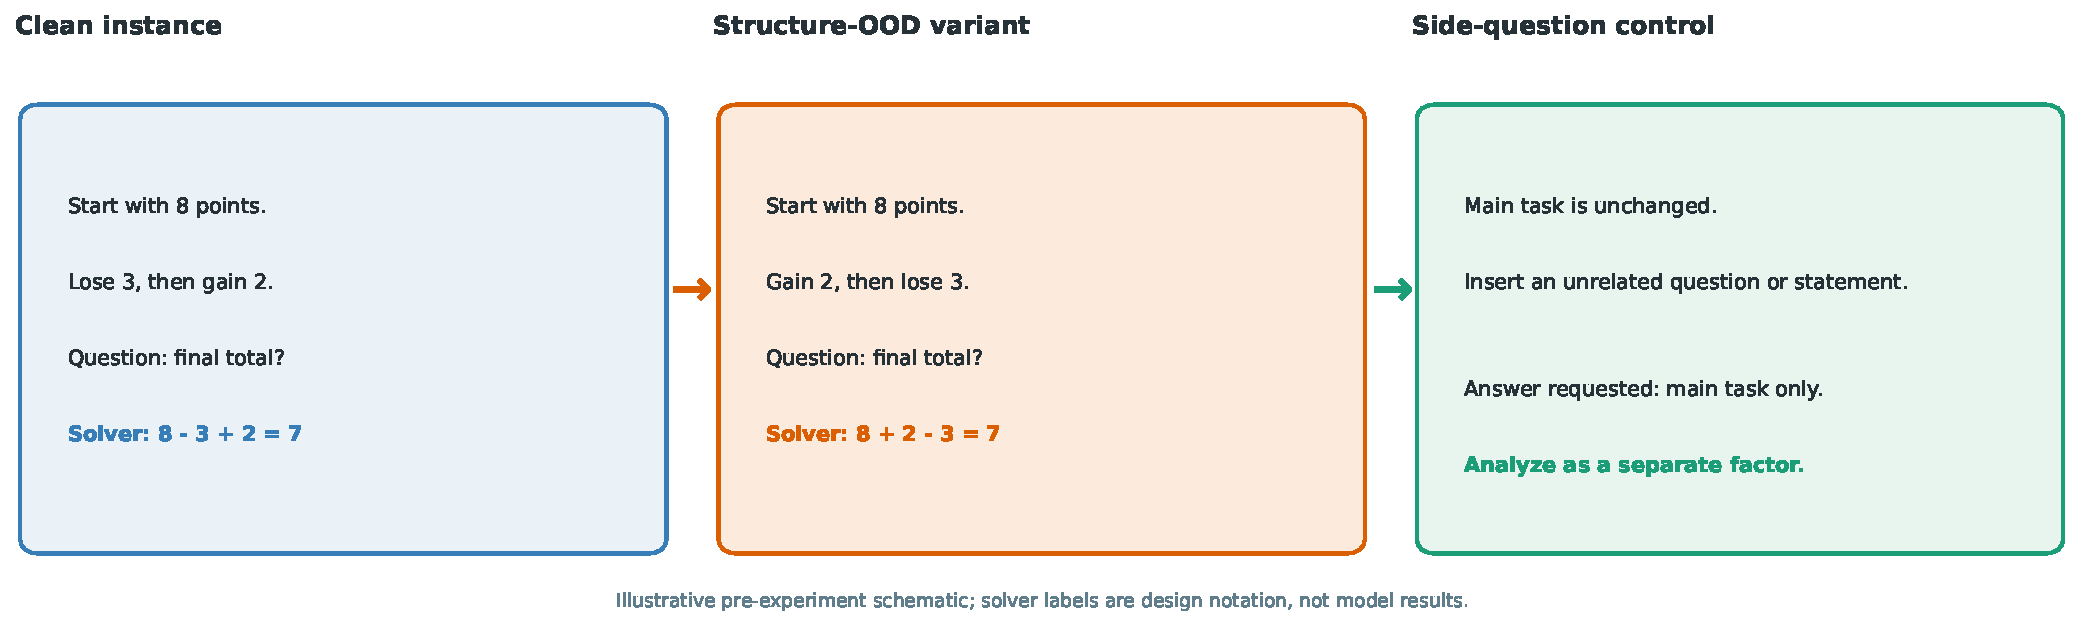
\includegraphics[width=\linewidth]{fig1_motivated_example.pdf}
  \caption{A solver-validated same-graph presentation change. The final figure
  will distinguish this stability pair from an independent unseen-graph
  transfer item.}
  \label{fig:motivation}
\end{figure}

\section{Related Work}

\paragraph{Compositional generalization.}
Compositionality work studies systematic transfer to unseen combinations
[1--4]. We adopt structural holdouts for final-answer reasoning while keeping
same-graph presentation stability as a separate estimand.

\paragraph{Reasoning robustness and context interference.}
GSM-Symbolic and GSM-Plus vary mathematical instances and clauses [5,6], while
other work studies irrelevant context and information position [7,8]. We treat
decoys and auxiliary questions as an interference pool rather than as direct
evidence of unseen dependency composition.

\paragraph{Rationales and adaptation.}
Noisy-rationale and faithfulness studies manipulate intermediate explanations
[9,10]. LoRA and QLoRA provide parameter-efficient adaptation [13,14], and
targeted adversarial training prioritizes current model errors [15]. We use
these ideas only for a matched boundary intervention; the scientific object is
the relationship between stability, transfer, and observable dependency burden.

\section{Stability and Transfer Framework}

\subsection{Problem formulation}

Represent a latent reasoning task as $z=(G,q,y)$, let $r$ denote its textual
realization, and let the model input be
\begin{equation}
x=R(z,r).
\end{equation}
Here $G$ is a dependency graph, $q$ is the target query, and $y$ is the
solver-verified answer. This notation separates the latent task from its
surface realization.

\subsection{Structural stability}

A stability transformation $T_s$ changes presentation while preserving the
graph, query, and answer:
\begin{equation}
G(T_sx)=G(x), \qquad q(T_sx)=q(x), \qquad y(T_sx)=y(x).
\end{equation}
Transformed accuracy mixes competence and stability. We therefore define the
conditional stability rate and flip rate as
\begin{equation}
SS(f)=\Pr[f(T_sx)=y\mid f(x)=y],
\qquad SF(f)=1-SS(f).
\end{equation}
The condition $f(x)=y$ asks whether a demonstrated solution survives an
equivalent presentation.
As a check against conditioning artifacts, we also report agreement between
two independently sampled equivalent realizations:
\begin{equation}
INV(f)=\mathbb E_{z,r,r'}\left[
\mathbf 1\{f(R(z,r))=f(R(z,r'))\}\right].
\end{equation}
Agreement can be high when a model consistently makes the same mistake, so it
does not replace $SS$.

\subsection{Structural transfer}

The transfer pool contains graph families or operator compositions excluded
from training, discovery, and stability pools. We compare risks over seen and
unseen graph distributions under the same canonical realization:
\begin{equation}
R_S(f)=\mathbb E_{G\sim P_S,q\sim P(q\mid G)}
\left[\mathbf 1\{f(x_G^{\mathrm{can}})\neq y_G\}\right],
\end{equation}
\begin{equation}
R_U(f)=\mathbb E_{G\sim P_U,q\sim P(q\mid G)}
\left[\mathbf 1\{f(x_G^{\mathrm{can}})\neq y_G\}\right].
\end{equation}
The canonical-presentation transfer gap is
\begin{equation}
\Delta_T(f)=
\Pr_{G\sim P_{\mathrm{seen}}}[f(x_G^{\mathrm{can}})=y_G]
-\Pr_{G\sim P_{\mathrm{unseen}}}[f(x_G^{\mathrm{can}})=y_G].
\end{equation}
The two graph distributions are matched on primitive operators, length, labels,
and templates. Unlike $SS$, $\Delta_T$ compares different graph supports under
the same presentation condition.
Equivalently, $\Delta_T=R_U-R_S$ is the increase in risk caused by changing
the graph support. We also report normalized transfer retention
\begin{equation}
TR(f)=1-\frac{R_U(f)-R_S(f)}{1-R_S(f)},\qquad R_S<1.
\end{equation}
Stability conditions on a fixed $z$ and varies $r$, whereas transfer fixes the
canonical realization and compares two distributions over $G$; there is no
identity linking the two quantities.

\subsection{A two-by-two decomposition}

Let $A_{g,p}$ denote accuracy for graph familiarity
$g\in\{\mathrm{seen},\mathrm{unseen}\}$ and presentation
$p\in\{\mathrm{canonical},\mathrm{shifted}\}$. We report
\begin{equation}
\Delta_S=A_{\mathrm{seen,canonical}}-A_{\mathrm{seen,shifted}},
\end{equation}
\begin{equation}
\Delta_T=A_{\mathrm{seen,canonical}}-A_{\mathrm{unseen,canonical}},
\end{equation}
and
\begin{equation}
I_{S\times T}=
\left(A_{\mathrm{seen,canonical}}-A_{\mathrm{seen,shifted}}\right)
-\left(A_{\mathrm{unseen,canonical}}-A_{\mathrm{unseen,shifted}}\right).
\end{equation}
These are stability, transfer, and interaction contrasts, respectively; they
are not relabeled versions of one score.

\subsection{Finite theorems for a closure solver}

The statements below are proved in Lean~4. Proofs are in
Appendix~\ref{app:proofs-en}. Each statement constrains a closure solver and
finite counterexamples. It is not a measurement of a trained model. Atoms are
natural numbers. A rule is a premise set implying a conclusion. The solver
answer is $y$. Order, synonym, premise deletion, and graph change are
$O_\sigma$, $L^{\equiv}$, $L^{\times}$, and $H_\psi$. Extraction is $\varphi$.
A closure solver is
\begin{equation}
f(x)=\mathbf{1}\{q\in\mathrm{Closure}(\varphi(x))\},
\end{equation}
with $\varphi(T_sx)=\varphi(x)$ for every stability transformation $T_s$.
When the fuel is at least the number of rules, closure membership coincides
with definite-clause derivation.

\begin{lemma}[Order and synonym]
\label{lem:order-en}
\begin{align}
y(O_\sigma\omega)&=y(\omega),\\
y(L^{\equiv}\omega)&=y(\omega).
\end{align}
Thus $O_\sigma$ and $L^{\equiv}$ are stability transformations. For the task
$\omega_0$ with an empty fact set, rule $\{0\}\to 1$, and query $1$,
\begin{equation}
y(\omega_0)=\mathrm{no},\qquad y(L^{\times}\omega_0)=\mathrm{yes},
\end{equation}
so $L^{\times}$ is not a stability transformation. $H_\psi$ replaces
$\{0\}\to 1$ by $\{0\}\to 2$. The two rule sets differ, so $H_\psi$ is not a
stability transformation either.
\end{lemma}

\begin{lemma}[Accuracy gap and flip counts]
\label{lem:gap-en}
Let each observation take $C,S\in\{0,1\}$. On every finite list,
\begin{equation}
\#\{C=1\}-\#\{S=1\}=\#\{C=1,S=0\}-\#\{C=0,S=1\}.
\end{equation}
Write $\Delta=\#\{C=1\}-\#\{S=1\}$, $N=\#\{C=1\}$,
$F=\#\{C=1,S=0\}$, and $R=\#\{C=0,S=1\}$. Then
\begin{equation}
\Delta\cdot N=FN-RN,
\qquad
SF=\frac{F}{N}\quad(N>0).
\end{equation}
Hence $\Delta=0$ does not imply $F=0$. The counterexample is two lists of
length $100$, both with $N=60$, and
\begin{equation}
SF\in\left\{0,\frac{30}{60}\right\}.
\end{equation}
\end{lemma}

\begin{lemma}[Seen-graph flips and the transfer gap]
\label{lem:worlds-en}
Two finite worlds $W_{=}$ and $W_{\neq}$, each of length $2$, satisfy
\begin{equation}
\#_{\mathrm{seen}}\{C=1\}=\#_{\mathrm{unseen}}\{C=1\}=2,
\qquad
\Delta_T(W_{=})=\Delta_T(W_{\neq})=0,
\end{equation}
while the seen-graph flip counts are
\begin{equation}
F(W_{=})=0,\qquad F(W_{\neq})=1.
\end{equation}
\end{lemma}

\begin{lemma}[Interaction and presentation differences]
\label{lem:interaction-en}
Over the integers,
\begin{align}
I_{S\times T}
&=(A_{\mathrm{sc}}-A_{\mathrm{ss}})-(A_{\mathrm{uc}}-A_{\mathrm{us}}),\\
J
&=(A_{\mathrm{ss}}-A_{\mathrm{us}})-(A_{\mathrm{sc}}-A_{\mathrm{uc}}),
\end{align}
and
\begin{equation}
I_{S\times T}=-J.
\end{equation}
\end{lemma}

\begin{lemma}[Inversions under full reversal]
\label{lem:inversion-en}
\begin{equation}
\operatorname{inv}(\mathrm{rev}(m))=\frac{m(m-1)}{2},
\qquad
\operatorname{inv}(\mathrm{id})=0.
\end{equation}
Therefore
\begin{equation}
\operatorname{inv}(\mathrm{rev}(2))=1\neq 3=\operatorname{inv}(\mathrm{rev}(3)).
\end{equation}
This is a combinatorial identity, not an experimental measurement.
\end{lemma}

\begin{theorem}[Orbits of a closure solver, and one counterexample function]
\label{thm:main-en}
If $\varphi\circ O_\sigma=\varphi$ and $\varphi\circ L^{\equiv}=\varphi$, then
on that orbit
\begin{equation}
f(x)=y\implies f(T_sx)=y,
\end{equation}
so $SS(f)=1$. If an unseen graph is still extracted correctly, then
\begin{equation}
f(x_U^{\mathrm{can}})=y
\qquad\text{and}\qquad
f(T_sx_U)=y.
\end{equation}
For the negative branch, a seen writing $\mathrm{seen}(t)$, $t\in\mathbb{N}$,
has rule $\{0\}\to 1$, fact $\{0\}$, and query $1$. The unseen canonical
writing has rule $\emptyset\to 2$, an empty fact set, and query $2$. The rule
sets are disjoint, and the solver answers $\mathrm{yes}$ on both. There is a
function
\begin{equation}
g(\mathrm{seen}(t))=\mathrm{yes},
\qquad
g(x_U^{\mathrm{can}})=\mathrm{no}.
\end{equation}
Thus $g$ is stable and correct on every writing of the seen graph, and
incorrect on that unseen item. Reorder training supported only on seen
writings does not exclude $g$.
\end{theorem}

\section{Predictive Dependency-Burden Law}

We test a task-level account in which some errors arise from dependency
tracking rather than length alone. Let $D_{\mathrm{rel}}(x)$ be the textual
distance among proof-relevant premises and let $F_{\mathrm{active}}(x)$ be the
maximum number of unresolved dependencies that must remain active before
combination. The candidate model is
\begin{equation}
\operatorname{logit}\Pr(e_{m,x}=1)
=\alpha_m+\beta_1D_{\mathrm{rel}}(x)
+\beta_2F_{\mathrm{active}}(x)+\gamma^\top Z(x),
\end{equation}
where $Z(x)$ controls length, graph size, target position, template, label,
depth, and branching. We choose the features, specification, and coefficient
directions on a discovery split and evaluate once on a protected confirmatory
split.

On the two-by-two data, we additionally fit
\begin{equation}
\operatorname{logit}\Pr(e_{m,x}=1)
=\alpha_m+\eta_S I_{\mathrm{shift}}(x)
+\eta_T I_{\mathrm{unseen}}(x)
+\eta_{ST}I_{\mathrm{shift}}(x)I_{\mathrm{unseen}}(x)
+\beta^\top X(x).
\end{equation}
The three coefficients represent presentation, unseen-graph, and interaction
effects. They keep stability and transfer as separate error increments rather
than collapsing them into one score.

\subsection{A concrete law and falsifiable predictions}

We do not call a correlation between the three structural features and error a
law. The primary confirmatory model retains the standardized feature vector:
\begin{equation}
\operatorname{logit}\Pr(e_{m,x}=1)
=\alpha_m+\beta_D\widetilde D_{\mathrm{rel}}(x)
+\beta_F\widetilde F_{\mathrm{active}}(x)
+\beta_K\widetilde K_{\mathrm{op}}(x)
+\gamma^\top Z(x).
\end{equation}
Only after freezing weights on discovery do we define a scalar burden summary
\begin{equation}
B(x)=w_D\widetilde D_{\mathrm{rel}}(x)
+w_F\widetilde F_{\mathrm{active}}(x)
+w_K\widetilde K_{\mathrm{op}}(x),
\qquad w_D,w_F,w_K\geq 0,
\end{equation}
and formulate the law as a conditional error risk:
\begin{equation}
\Pr(e_{m,x}=1\mid B(x),Z(x))
=\sigma\left(\alpha_m+\phi(B(x))+\gamma^\top Z(x)\right),
\end{equation}
where $Z(x)$ controls length, graph size, depth, branching, target position,
and template. The feature coefficients and any summary weights are frozen on
discovery; a fixed monotone spline is used only for shape checking.

The falsifiable predictions are that the feature directions are preserved,
higher frozen $B$ yields higher error risk after conditioning on $Z$, the
burden model outperforms the strongest length/graph-complexity baseline, and
binned error rates increase monotonically with burden. Direction reversal,
loss of predictive advantage, nonmonotone bins, or equal effects from matched
placebo hints restrict the claim to an exploratory trend.

The account is weakened if local subproblems fail at the same rate as full
proofs, nuisance-only models predict equally well, coefficient directions
reverse on confirmation, or dependency hints and matched placebo hints have
the same effect. The law is an observable prediction model, not a direct claim
about hidden neural states.

\section{Measurement Instrument}

StructShift creates three pools. The stability pool contains legal
same-graph ordering and rendering changes. The transfer pool contains unseen
graph families and operator compositions. Decoys and auxiliary questions form a
separate interference pool. Symbolic objects are split before rendering, and
each candidate is re-solved. Worlds, base-query IDs, graph hashes, graph-family
IDs, proof traces, relevant-premise positions, active frontier size, token
length, target position, template, and transformation lineage are retained.

\begin{figure}[t]
  \centering
  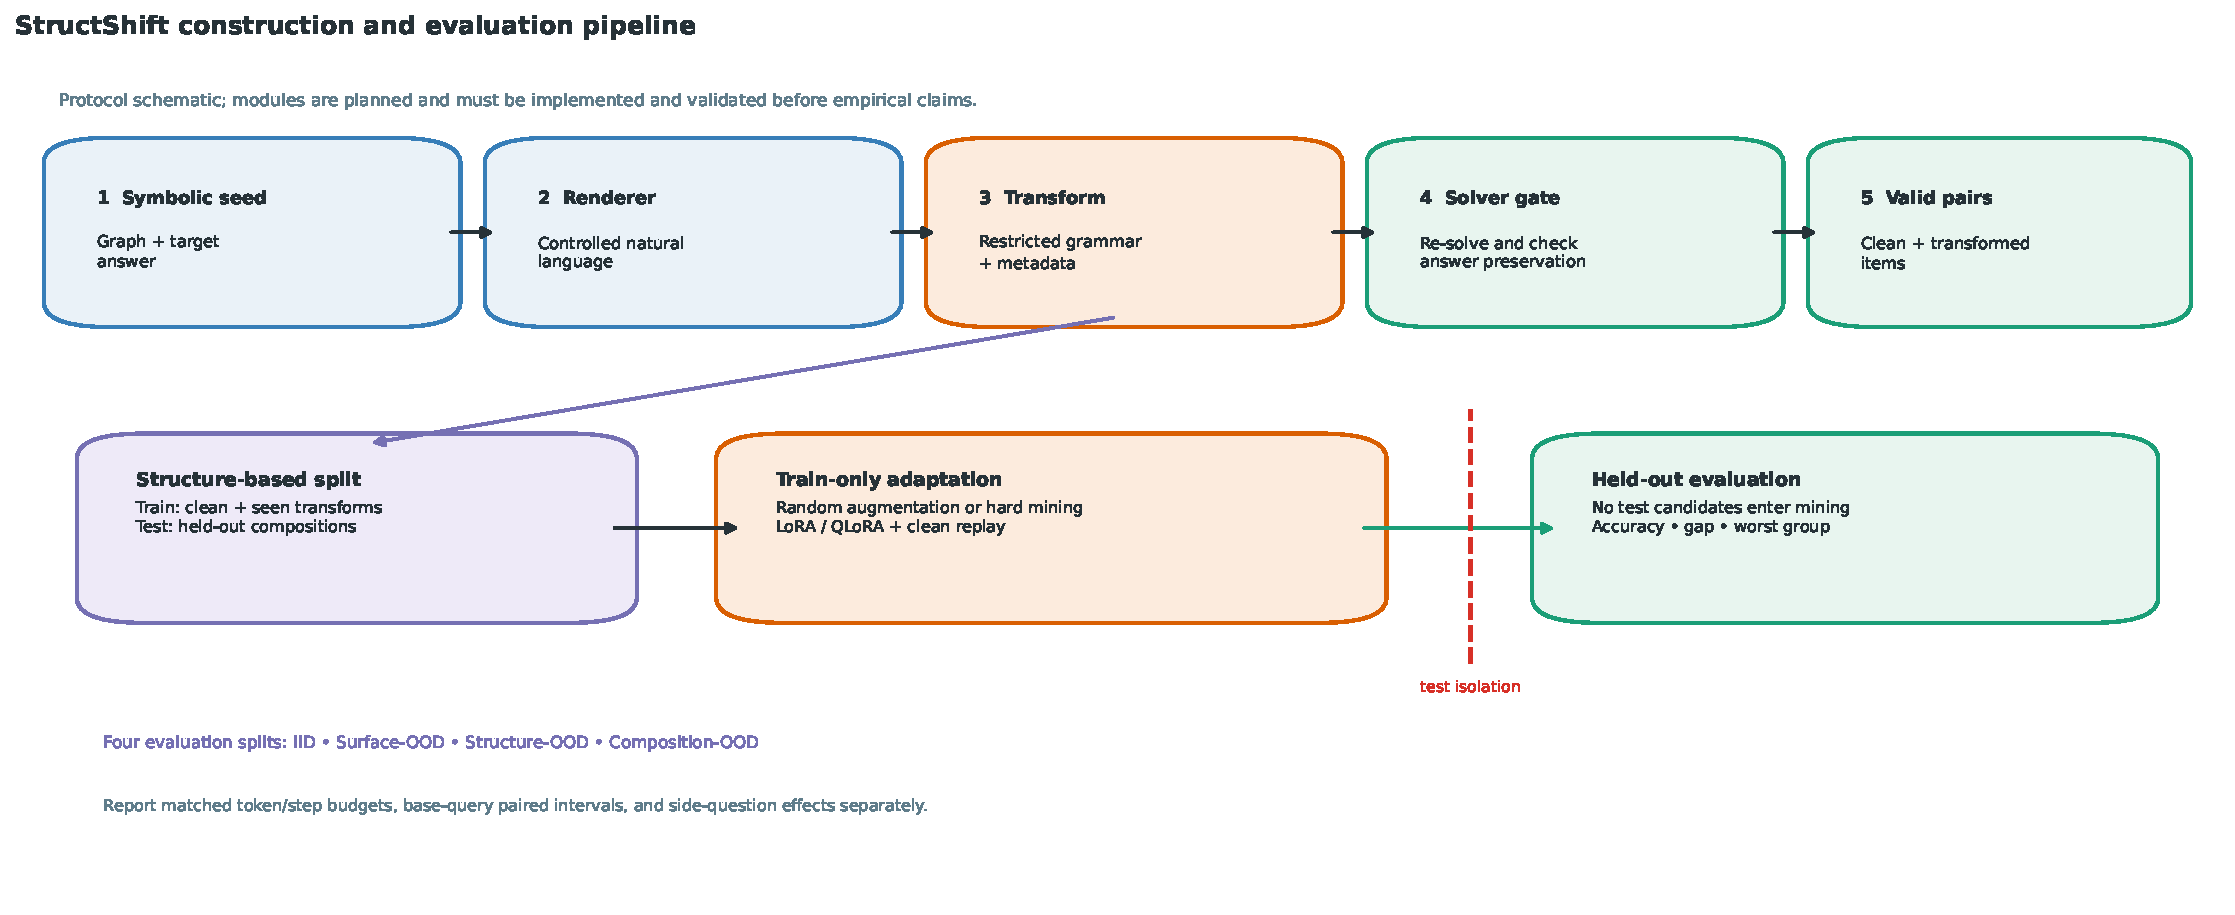
\includegraphics[width=\linewidth]{fig2_pipeline.pdf}
  \caption{Solver-validated construction and protected symbolic partitioning.
  This is a pre-experiment schematic.}
  \label{fig:pipeline}
\end{figure}

\section{Experimental Evidence Chain}

\subsection{E1: Structural stability}

We evaluate canonical and same-graph variants with deterministic decoding.
Increasing depth, branching, or changing operator composition is excluded from
the stability definition. We report clean accuracy, transformed accuracy,
conditional stability, conditional flips, recovery, and paired bootstrap
intervals.

\subsection{E2: Structural transfer}

We evaluate held-out graph families and operator compositions under canonical
presentation. Stability and transfer pools share no worlds, base queries, graph
hashes, or graph families. Their relationship is tested only across multiple
models, checkpoints, or controlled training conditions, while controlling
independently measured clean competence.

\subsection{E2.5: Orthogonal intervention and double dissociation}

We compare four matched training conditions: Base, Render-Aug with only
same-graph equivalent realizations, Graph-Aug with only canonical new graph
compositions, and Joint with both. All conditions are evaluated on the same
two-by-two cells and matched for training tokens, steps, LoRA rank, target
modules, random seeds, and compute.

Define gains over Base as
\begin{equation}
G_S(c)=SS_c-SS_{\mathrm{Base}},\qquad
G_T(c)=\Delta_{T,\mathrm{Base}}-\Delta_{T,c}.
\end{equation}
Render-Aug supports a stability-specific effect only when $G_S$ exceeds a
pre-registered margin while $G_T$ falls inside the transfer equivalence margin;
Graph-Aug uses the reverse criterion. Equivalence intervals are required
instead of interpreting one significant and one nonsignificant result as
dissociation.

\subsection{E3: Out-of-sample error prediction}

We compare length-only, graph-complexity-only, depth/branching, and full
dependency-burden models. Confirmatory evaluation reports held-out log loss or
Brier score, calibration, rank correlation, and error by burden bin. Local
subquestions and dependency/placebo hints provide discriminating controls.

\section{Applicability Boundary}

Represent a test condition as
\begin{equation}
\tau=(\mathcal G,\mathcal R,\mathcal Q,m,d),
\end{equation}
for graph distribution, realization distribution, task family, model, and
decoding condition. After freezing the feature algorithms, normalization
parameters, model specification, and coefficient directions on discovery, we
define
\begin{equation}
V(\tau)=
\bigl(
V_{\mathrm{direction}}(\tau),
V_{\mathrm{prediction}}(\tau),
V_{\mathrm{calibration}}(\tau)
\bigr).
\end{equation}
The applicability domain is
\begin{equation}
\mathcal A=\{\tau:V_{\mathrm{direction}}(\tau)=V_{\mathrm{prediction}}(\tau)=V_{\mathrm{calibration}}(\tau)=1\}.
\end{equation}
Boundary experiments change one main factor at a time and record the task
family, graph distribution, realization rule, model, intervention, and the
three separate verdicts. This turns applicability into a measurable domain
rather than a single second-task accuracy.

\section{Boundary and Intervention}

We repeat the frozen analysis on a second reasoning family with new templates
and vocabulary. Only then do we compare a frozen base, clean-only LoRA, random
legal structural augmentation, and optional error-guided structural LoRA under
matched rank, target modules, tokens, steps, labels, seeds, and compute. Gains
only on seen variants are local adaptation. Gains on protected transfer are
intervention evidence, but do not alone prove a hidden neural mechanism.

\subsection{Pre-experiment pipeline validation}

Before connecting a language model, we ran a minimal validation of the data
construction and metric pipeline. With random seed 20261008, we generated 25
symbolic graphs per family for two seen families (chain and fork\_join) and two
held-out families (chain\_then\_fork and double\_chain\_join), yielding 200
canonical/shifted records. Each shifted record changes only the presentation
order of premises on the same dependency graph, and its solver answer must
match the canonical answer. Held-out families are isolated at the symbolic
level and do not enter the stability or discovery pool.

This check verifies the generator, answer-preservation checks for equivalent
realizations, graph-family splitting, and metadata recording. Four unit tests
cover pairing, answer preservation, and seen/unseen family isolation. These
results establish only that the measurement pipeline runs as specified; they
are not evidence about language-model robustness. Model accuracy, $SS$, $SF$,
and $\Delta_T$ will be reported after real-model predictions are connected.

We also ran a non-confirmatory exploratory pilot with Qwen2.5-1.5B-Instruct on
the same 200 records. Accuracy was 0.76 in all four cells, with $SS=1.00$ and
$\Delta_T=0.00$. Each cell, however, contains 38 ``yes'' and 12 ``no'' labels,
and the model almost always outputs ``yes''. Thus 0.76 is the label baseline,
while $SS=1.00$ means only that the canonical and shifted outputs did not flip;
neither result supports a structural-robustness claim. The confirmatory pilot
must balance labels, randomize evaluation order, and include deeper, branched,
and held-out compositions that produce measurable model errors.

\begin{table}[t]
  \centering
  \caption{Exploratory Qwen2.5-1.5B-Instruct pilot. Each cell contains 50
  examples; label imbalance makes this a pipeline check rather than a
  confirmatory result.}
  \label{tab:pilot}
  \begin{tabular}{lcc}
    \toprule
    Cell & $n$ & Accuracy \\
    \midrule
    Seen graph / canonical & 50 & 0.76 \\
    Seen graph / shifted & 50 & 0.76 \\
    Unseen graph / canonical & 50 & 0.76 \\
    Unseen graph / shifted & 50 & 0.76 \\
    \midrule
    Conditional stability $SS$ & -- & 1.00 \\
    Transfer gap $\Delta_T$ & -- & 0.00 \\
    \bottomrule
  \end{tabular}
\end{table}

\begin{figure}[t]
  \centering
  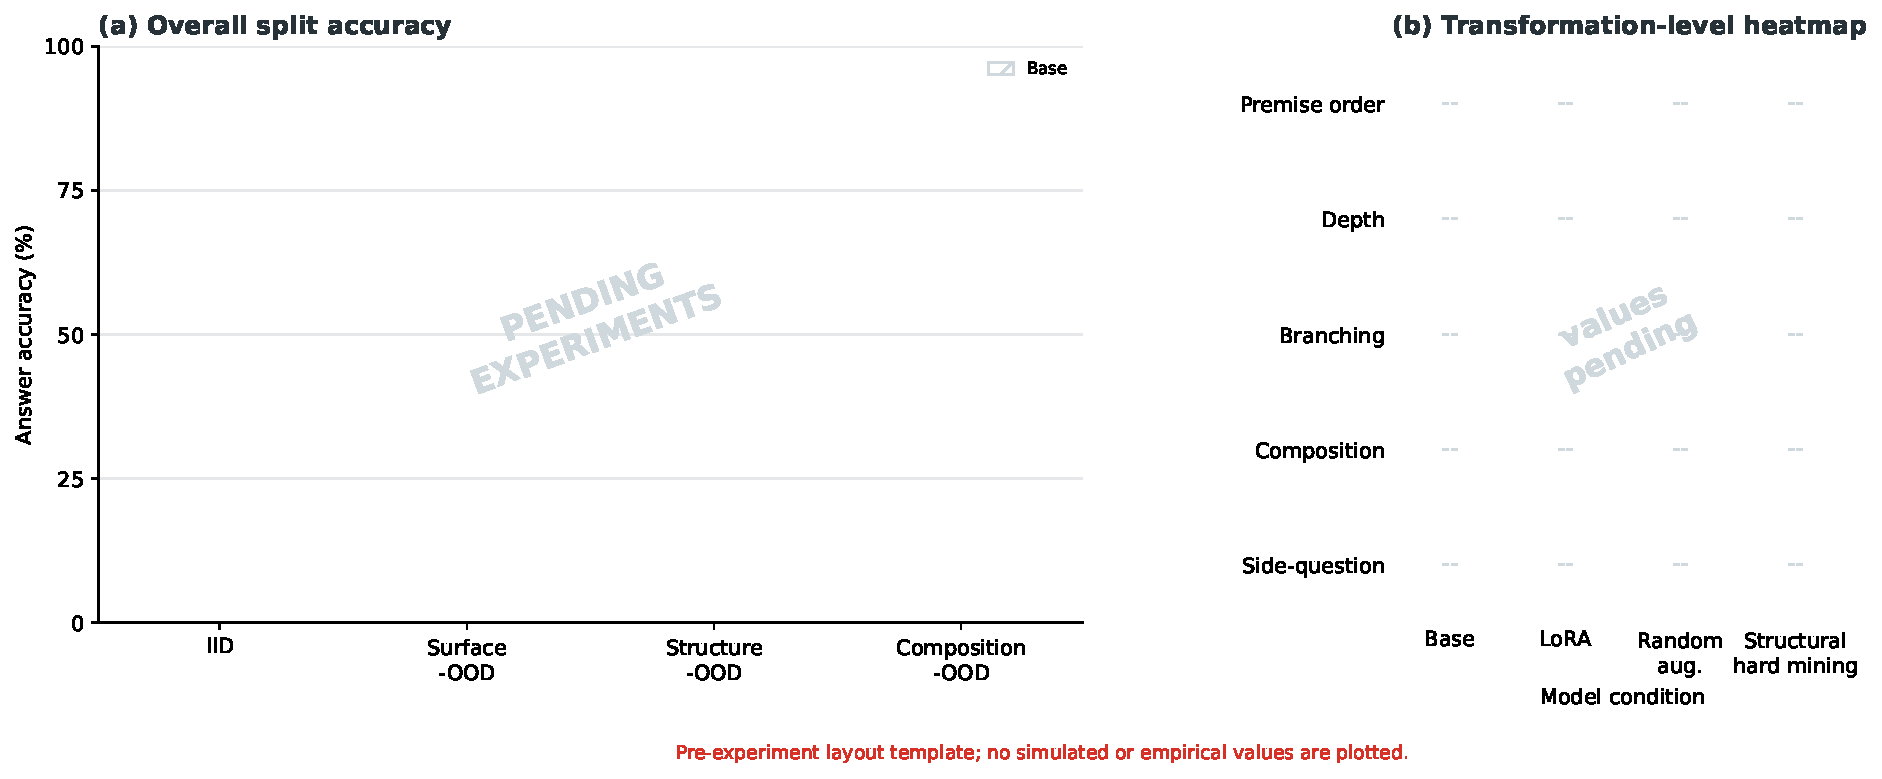
\includegraphics[width=\linewidth]{fig3_results_template.pdf}
  \caption{Planned result layout for stability, transfer, error prediction, and
  boundary tests. Values are filled after real-model experiments.}
  \label{fig:results}
\end{figure}

\section{Discussion and Limitations}

The stability definition covers only presentation changes that preserve the
same graph. Transfer depends on strict graph-family holdouts; weak holdouts can
make surface changes look like structural transfer. The dependency law is a
task-level predictive account and does not identify internal model states.
Cross-model association between stability and transfer is not causal by itself.
An intervention that improves only seen variants must be reported as local
adaptation.

\section{Conclusion}

This paper separates structural stability from structural transfer in reasoning.
The first is conditional answer preservation on the same graph; the second is
performance on unseen dependency graphs under canonical presentation. A
solver-validated measurement instrument, a frozen dependency-burden law, and
independent-task and intervention tests together determine whether the observed
pattern is stable, predictive, transferable, or task-specific.

\appendix
\section{Proofs for the closure solver and finite counterexamples}
\label{app:proofs-en}

The development is the Lake project \texttt{proof/StructRobust}, checked with
Lean~4.35.0 and the core library only, without mathlib. The text below
restates the arguments and does not paste tactic scripts. Each item is a
theorem about a closure solver and finite counterexamples, not a measurement
of a trained model.

\subsection{Closure}
\label{app:closure-en}

File \texttt{proof/StructRobust/StructRobust/Closure.lean}, theorem
\texttt{closure\_fuel\_iff\_derives}. One round folds the rule list: if every
premise is already known and the conclusion is not, the conclusion is added.
Fuel $k+1$ performs $k$ rounds and then one more fold. Definite-clause
derivation, \texttt{Derives}, has two clauses. A fact is derivable. If a rule
belongs to the rule set and every premise is derivable, the conclusion is
derivable.

Soundness is induction on fuel. A round adds the head of a rule whose premises
are already known, so the new atom remains derivable from the original facts
and rules. Completeness uses a potential: the number of rules whose heads are
still missing. The potential is at most the number of rules. If a round does
not reach a closed set, it adds at least one new head and the potential
strictly decreases. Thus fuel at least the length of the rule list reaches a
fixpoint, and every derivable atom has entered the closure. The solver accepts
a query exactly when the query lies in that closure; see
\texttt{solver\_iff\_derives} in \texttt{Operators.lean}.

\subsection{Lemma~\ref{lem:order-en}}

File \texttt{proof/StructRobust/StructRobust/Operators.lean}.

Order. Theorem \texttt{lemma1\_order\_preserves}: if two rule lists have the
same members, \texttt{Derives} holds on one side exactly when it holds on the
other, because a derivation uses only membership in the set
(\texttt{derives\_rules\_congr} in \texttt{Closure.lean}). Theorem
\texttt{lemma1\_reorder\_stable}: replacing the list while preserving
membership leaves the fact set, the rule set, and the query unchanged, so the
operator is a stability transformation \texttt{IsStability}. Theorem
\texttt{stability\_preserves} says every such transformation preserves the
solver answer.

Synonym. A \texttt{Phrase} is a rule plus one wrapping field. Theorem
\texttt{lemma1\_synonym\_denote}: changing the wrap does not change the
denotation. Theorem \texttt{lemma1\_synonym\_extract}: extraction maps each
phrase to its denotation, so wrapping every phrase leaves the extracted rule
list unchanged.

Ambiguity. Theorem \texttt{lemma1\_ambiguity\_changes}. The task has no facts,
one rule with premise $0$ and head $1$, and query $1$. There is no fact to
start from, and the only rule demands premise $0$, so no atom is derivable.
After the premise is deleted, the rule has an empty premise list and head $1$,
so $1$ is derivable. The answers differ. Theorem
\texttt{lemma1\_ambiguity\_not\_stability}: a stability transformation would
have preserved the answer.

Graph change. Theorem \texttt{lemma1\_graph\_not\_stability}. One task has the
rule $\{0\}\to 1$ and the other has $\{0\}\to 2$. The first rule is not a
member of the second rule set, so the finite sets differ and the pair is not a
stability transformation.

\subsection{Lemma~\ref{lem:gap-en}}

File \texttt{proof/StructRobust/StructRobust/Counting.lean}. An observation is
a pair of Booleans. Split $\#\{C=1\}$ into the cells $S=0$ and $S=1$, and split
$\#\{S=1\}$ into the cells $C=0$ and $C=1$. Subtracting cancels the shared cell
$\#\{C=1,S=1\}$ and yields theorem \texttt{lemma2\_count\_gap}. Theorem
\texttt{lemma2\_gap\_times\_correct} multiplies both sides by $\#\{C=1\}$ and
distributes. The subtracted term is $\#\{C=0,S=1\}$, the items that are wrong
in the canonical writing and right after the transformation.

The two populations are concatenations of repeated observations. Theorem
\texttt{lemma2\_stable\_counts}: sixty copies of $(C,S)=(1,1)$ followed by
forty copies of $(0,0)$ have length $100$, sixty canonical successes, sixty
transformed successes, and flip count $0$. Theorem
\texttt{lemma2\_flip\_counts}: thirty copies each of $(1,1)$, $(1,0)$, and
$(0,1)$, plus ten copies of $(0,0)$, also have length $100$ and sixty canonical
successes, of which thirty flip. Theorem
\texttt{lemma2\_same\_accuracy\_different\_sf} records both populations
together. Accuracy is $60/100$ in each, while the flip counts are $0$ and
$30$. Relative to the sixty canonically correct items, the conditional flip
ratios are $0$ and $30/60$. The argument uses only finite counting.

\subsection{Lemma~\ref{lem:worlds-en}}

File \texttt{proof/StructRobust/StructRobust/Worlds.lean}, theorem
\texttt{lemma3\_same\_transfer\_different\_sf}. In the first world the seen
list is two copies of $(1,1)$ and the unseen canonical marks are two truths.
In the second world the seen list is one $(1,0)$ and one $(1,1)$, and the
unseen marks are again two truths. Both worlds have two canonically correct
seen items and two canonically correct unseen items, so both transfer gaps are
$0$. The seen-graph flip counts are $0$ and $1$, with denominator $2$ in each
world. The canonical transfer gap can therefore agree while the seen-graph
flip count does not.

\subsection{Lemma~\ref{lem:interaction-en}}

File \texttt{proof/StructRobust/StructRobust/Interaction.lean}, theorem
\texttt{lemma4\_interaction\_opposite}. Expand
\[
I=(A_{\mathrm{sc}}-A_{\mathrm{ss}})-(A_{\mathrm{uc}}-A_{\mathrm{us}})
\]
and
\[
J=(A_{\mathrm{ss}}-A_{\mathrm{us}})-(A_{\mathrm{sc}}-A_{\mathrm{uc}})
\]
over the integers. Then
$I=A_{\mathrm{sc}}-A_{\mathrm{ss}}-A_{\mathrm{uc}}+A_{\mathrm{us}}$ and
$J=-A_{\mathrm{sc}}+A_{\mathrm{ss}}+A_{\mathrm{uc}}-A_{\mathrm{us}}$. Their sum
is $0$, so $I=-J$.

\subsection{Lemma~\ref{lem:inversion-en}}

File \texttt{proof/StructRobust/StructRobust/Inversion.lean}. An inversion
count adds, for each entry, the number of strictly smaller entries after it.
The sorted list \texttt{canonOrder} is $0,1,\ldots,m-1$. Every later entry is
larger, so theorem \texttt{lemma5\_canon\_inversions} gives inversion count
$0$. The reversed list \texttt{revOrder} is $m-1,\ldots,0$. In the inductive
step, the list of length $m+1$ places $m$ first. That entry is larger than
each of the $m$ entries after it, and the tail is the reversal of length $m$.
The inversion counts therefore satisfy $a_{m+1}=a_m+m$ with $a_0=0$, hence
$2a_m=m(m-1)$. Theorem \texttt{lemma5\_reverse\_inversions} divides by $2$ and
obtains $m(m-1)/2$. Theorems \texttt{lemma5\_reverse\_two} and
\texttt{lemma5\_reverse\_three} evaluate the count at $m=2$ and $m=3$, giving
$1$ and $3$. Theorem \texttt{lemma5\_reverse\_two\_ne\_three} records that
these two doses differ. The count depends only on the permutation. It is not a
measurement of model output.

\subsection{Positive branch of Theorem~\ref{thm:main-en}}

File \texttt{proof/StructRobust/StructRobust/Main.lean}. The function
\texttt{fAnswer} extracts rules from the surface phrases and asks whether the
query lies in the closure of that rule list. Theorem
\texttt{main\_positive\_orbit}: if two surfaces extract the same set of rules,
closure membership agrees, so $f$ equals the solver answer on the canonical
extraction. Theorem \texttt{main\_positive\_reorder}: if two phrase lists have
the same members, their extracted rule sets agree, and reordering does not
change $f$. Theorem \texttt{main\_positive\_synonym}: wrapping every phrase
leaves the extracted list identical, so a synonym does not change $f$. Theorem
\texttt{main\_positive\_finite\_ss}: if $f$ holds on the canonical writing and
the transformed extraction is the same rule set, then $f$ holds after the
transformation. Theorem \texttt{main\_positive\_finite\_ss\_all} applies this
to every item of a finite list: every canonically correct item remains correct
after the transformation. Theorem \texttt{main\_positive\_unseen}: if the
canonical extraction of an unseen item already derives the query, then both
the canonical writing and any writing with the same extracted rule set are
correct.

\subsection{Negative branch of Theorem~\ref{thm:main-en}}

The same file. A writing of the seen graph carries a natural-number tag. Its
facts are $[0]$, its rule is $\{0\}\to 1$, and its query is $1$. The fact $0$
fires the rule, so $1$ is derivable (\texttt{seen\_derives}). The function
\texttt{fArbitrary} returns true on every seen tag. Theorem
\texttt{main\_negative\_seen\_correct} says this matches the solver. Theorem
\texttt{main\_negative\_seen\_stable} says any two tags receive the same
value, so every writing of the seen graph agrees. The unseen item has no
facts, a rule with no premises and head $2$, and query $2$. The empty-premise
rule derives $2$ (\texttt{unseen\_derives}), so the solver answer is true.
\texttt{fArbitrary} returns false on that item. Theorem
\texttt{main\_negative\_unseen\_incorrect} says the function disagrees with
the solver. Theorem \texttt{main\_negative\_disjoint}: the seen rule
$\{0\}\to 1$ is not a member of the unseen rule set, so the two rule sets are
disjoint and the unseen item is not a writing of the seen graph. Stability and
correctness on the seen graph do not yield correctness on that unseen item.

\begin{thebibliography}{99}
\bibitem{hupkes2020} D. Hupkes, V. Dankers, M. Mul, and E. Bruni. Compositionality Decomposed: How Do Neural Networks Generalise? JAIR, 2020.
\bibitem{oren2020} J. Oren et al. Improving Compositional Generalization in Semantic Parsing. Findings of EMNLP, 2020.
\bibitem{herzig2021} J. Herzig and J. Berant. Span-based Semantic Parsing for Compositional Generalization. ACL-IJCNLP, 2021.
\bibitem{qiu2022} L. Qiu et al. Evaluating the Impact of Model Scale for Compositional Generalization in Semantic Parsing. EMNLP, 2022.
\bibitem{mirzadeh2024} I. Mirzadeh et al. GSM-Symbolic: Understanding the Limitations of Mathematical Reasoning in Large Language Models. arXiv, 2024.
\bibitem{li2024} Q. Li et al. GSM-Plus: A Comprehensive Benchmark for Evaluating the Robustness of LLMs as Mathematical Problem Solvers. ACL, 2024.
\bibitem{shi2023} F. Shi et al. Large Language Models Can Be Easily Distracted by Irrelevant Context. arXiv, 2023.
\bibitem{liu2024} N. F. Liu et al. Lost in the Middle: How Language Models Use Long Contexts. TACL, 2024.
\bibitem{zhou2024} Z. Zhou et al. Can Language Models Perform Robust Reasoning in Chain-of-thought Prompting with Noisy Rationales? NeurIPS, 2024.
\bibitem{paul2024} D. Paul et al. Making Reasoning Matter: Measuring and Improving Faithfulness of Chain-of-Thought Reasoning. Findings of EMNLP, 2024.
\bibitem{press2023} O. Press et al. Measuring and Narrowing the Compositionality Gap in Language Models. Findings of EMNLP, 2023.
\bibitem{jia2017} R. Jia and P. Liang. Adversarial Examples for Evaluating Reading Comprehension Systems. EMNLP, 2017.
\bibitem{hu2022} E. J. Hu et al. LoRA: Low-Rank Adaptation of Large Language Models. ICLR, 2022.
\bibitem{dettmers2023} T. Dettmers et al. QLoRA: Efficient Finetuning of Quantized Language Models. NeurIPS, 2023.
\bibitem{pereira2021} J. Pereira et al. Targeted Adversarial Training for Natural Language Understanding. NAACL, 2021.
\end{thebibliography}
\end{document}
